\documentclass[11pt,a4paper]{article}
\usepackage[T1]{fontenc}
\usepackage[margin=2.3cm]{geometry}
\usepackage{amsmath,amssymb}
\usepackage{graphicx}
\usepackage[dvipsnames]{xcolor}
\usepackage{enumitem}
\usepackage[colorlinks=true,linkcolor=blue,urlcolor=blue]{hyperref}
\setlength{\parskip}{0.6em}
\setlength{\parindent}{0pt}
\begin{document}

\begin{center}{\LARGE\bfseries openreactionrate}\\[0.4em]{\large Write reaction networks as equations and watch catalysts speed them up, in three sessions.}\\[0.2em]\small PAN IIT OSS explainer \textbullet{} secondary school to diploma / undergraduate (levels 3-5)\end{center}

\section*{Why this exists}
Chemical reactions are processes in time: some are over in a flash, some take years. This explainer shows how the speed of a reaction is written as an equation, how temperature and a catalyst change it, and how a whole network of reactions becomes a set of differential equations that a computer can solve.

\section*{The end goal}
Write reaction networks as ODEs and see how catalysts speed them. The end goal is to write reaction networks as ODEs and see how catalysts speed them. The same mathematics describes enzymes, atmospheric chemistry, combustion and drug breakdown, but our models are simplified teaching models and not design tools.

\section*{How the three sessions build up}
\begin{enumerate}[nosep]
\item \textbf{Session 1: Reactions take time: concentration against time} (Level 1, conceptual interactive model, 60 min).
\item \textbf{Session 2: Rate laws, temperature and catalysts} (Level 2, mathematical engineering model, 75 min).
\item \textbf{Session 3: Reaction networks as ODEs, and when they bite back} (Level 3, simulation and validation, 90 min).
\end{enumerate}

\section{Session 1: Reactions take time: concentration against time}

\subsection*{A. Real-world problem}
Milk sours in a day on the kitchen table and in a week in the fridge. A bottle of hydrogen peroxide keeps for months, but a pinch of manganese dioxide makes it fizz at once. Chemical reactions take time, and some things (warmth, more molecules in the same space, a catalyst) change how much time. How can we draw, and then predict, how fast a substance A turns into a substance B?

\subsection*{B. Concept and theory}
For a molecule of A to turn into B it usually has to collide with something, and the collision must be energetic enough. If there are more A molecules in the same volume (a higher concentration) there are more collisions per second, so the rate is bigger. In the simplest reaction A -\textgreater{} B the rate (how many mol/L of A disappear per second) is proportional to the concentration of A: rate = k [A]. The constant k is the rate constant; a big k means a fast reaction. Warming the mixture makes collisions more frequent and, much more importantly, more energetic, so k grows. A catalyst gives the reaction an easier route, which also raises k, and it is not used up. Solving rate = k [A] gives an exponential decay: [A] falls fast at first, when there is a lot of A, and then more slowly. The half-life is the time for [A] to halve; for this reaction it is the same wherever you start. B is simply what A has lost, [B] = A0 - [A]. Here the catalyst is modelled in the simplest way, as a factor f that multiplies k.

\begin{itemize}[nosep]
\item [A]: concentration of A at time t (mol/L)
\item A0: starting concentration of A (mol/L)
\item k: rate constant (for A -\textgreater{} B) (1/s)
\item t: time (s)
\item t\_half: half-life: time for [A] to halve (s)
\item f: catalyst speed-up factor (k is multiplied by f) (no unit)
\end{itemize}

\begin{equation*}
\text{rate}=-\frac{d[A]}{dt}=k\,[A]
\end{equation*}

\begin{equation*}
[A]_t=A_0\,e^{-kt},\qquad [B]_t=A_0-[A]_t
\end{equation*}

\begin{equation*}
t_{1/2}=\frac{\ln 2}{k},\qquad t_{x}=\frac{1}{k}\ln\frac{1}{1-x}\ \ (\text{time to convert a fraction }x)
\end{equation*}

\begin{center}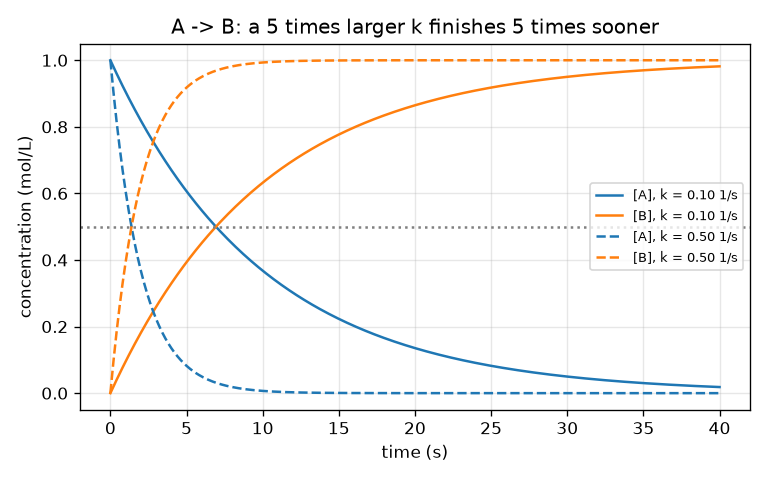
\includegraphics[width=0.85\linewidth]{figures/s01_a_to_b.png}\\\small [A] and [B] for A -\textgreater{} B; the 5 times catalyst (dashed) squeezes the same curve into one fifth of the time.\end{center}

\subsection*{E. Worked example}
For A -\textgreater{} B with k = 0.10 1/s and A0 = 1.0 mol/L, find [A] and [B] after 10 s, the half-life, and the time to convert 90 percent. Then see what a catalyst that makes k five times larger does to the last number.
\begin{enumerate}[nosep]
\item [A] after 10 s: k t = 0.10 * 10 = 1.0, so [A] = 1.0 * exp(-1.0) = 0.368 mol/L.
\item [B] = A0 - [A] = 1.0 - 0.368 = 0.632 mol/L. (Check: A + B = 1.000 mol/L.)
\item Half-life = ln 2 / k = 0.693 / 0.10 = 6.93 s.
\item 90 percent converted means [A] = 0.10: t = ln(10) / k = 2.303 / 0.10 = 23.0 s.
\item With the catalyst k = 0.50 1/s, so the time is 2.303 / 0.50 = 4.6 s: five times sooner.
\end{enumerate}
\textbf{Answer.} [A] = 0.368 mol/L and [B] = 0.632 mol/L after 10 s; half-life 6.93 s; 90 percent after 23.0 s, or 4.6 s with the 5 times catalyst.

\subsection*{F. Questions}
\begin{enumerate}[nosep]
\item \textbf{Conceptual.} Why does the concentration of A fall quickly at first and slowly later, even though nothing about the reaction changes?
\item \textbf{Numerical.} A reaction A -\textgreater{} B has k = 0.05 1/s and A0 = 2.0 mol/L. Find [A] after 20 s and the half-life, and check your answer for sense.
\item \textbf{Graph and simulation interpretation.} On the A-B graph of the slider app (A0 = 1, k = 0.10), where do the curves cross and what value do they have there? What would change if A0 were 2?
\item \textbf{Design and optimisation challenge.} Design: a reaction with k = 0.10 1/s must be 90 percent complete within 10 s. By what factor must a catalyst raise k? Which whole-number factor would you choose, and what other things besides speed matter?
\end{enumerate}

\section{Session 2: Rate laws, temperature and catalysts}

\subsection*{A. Real-world problem}
Someone has to decide how long a reaction must run, at what temperature, and whether a catalyst is worth it. For that we need an equation for the rate, a way to tell from measurements what kind of reaction it is, and the effect of temperature and of a catalyst on k. A common rule of thumb says 'a reaction goes about twice as fast for every 10 degrees warmer'. Is that rule right, and what does a catalyst do compared with warming? (General education only: real process design needs measured data and a safety review.)

\subsection*{B. Concept and theory}
A rate law says how the rate depends on concentration: rate = k [A]\textasciicircum{}n. The exponent n is the order, found from experiments, not from the equation of the reaction. For n = 1 the half-life ln 2 / k does not depend on the start; for n = 2 the half-life is 1 / (k A0) and gets longer as A is used up. You can read the order from data by choosing the plot that gives a straight line: ln[A] against t for first order (slope -k), 1/[A] against t for second order (slope +k). Temperature enters through k. Only collisions with energy above the activation energy Ea can react, and the share of such collisions grows steeply with temperature: k = A exp(-Ea / R T), the Arrhenius form (R = 8.314 J/(mol K), T in kelvin, A the pre-exponential factor with the units of k). Comparing two temperatures, A cancels: k(T2)/k(T1) = exp(-Ea/R (1/T2 - 1/T1)). A catalyst gives another route with a lower activation energy, Ea - dEa, so at the same temperature k is multiplied by exp(dEa / (R T)). Because Ea sits in an exponent, a modest drop gives a huge speed-up. Whether a reaction releases heat (exothermic: the products sit lower in energy than the reactants) or absorbs heat (endothermic: higher) is a separate matter from how high the barrier is. Estimating Ea carefully from measured data is the job of the openarrhenius repo.

\begin{itemize}[nosep]
\item n: order of the reaction (no unit)
\item k: rate constant (1/s (n = 1), L/(mol s) (n = 2))
\item A0, [A]: starting and current concentration (mol/L)
\item Ea: activation energy (J/mol)
\item R: gas constant, 8.314 (J/(mol K))
\item T: absolute temperature (K)
\item dEa: drop in activation energy caused by a catalyst (J/mol)
\item x: fraction converted (0 to 1) (no unit)
\end{itemize}

\begin{equation*}
[A]_t=A_0e^{-kt}\ (n=1),\qquad t_{1/2}=\frac{\ln 2}{k}
\end{equation*}

\begin{equation*}
[A]_t=\frac{A_0}{1+kA_0t}\ (n=2),\qquad t_{1/2}=\frac{1}{kA_0}
\end{equation*}

\begin{equation*}
\ln[A]=\ln A_0-kt\ (n=1),\qquad \frac{1}{[A]}=\frac{1}{A_0}+kt\ (n=2)
\end{equation*}

\begin{equation*}
k=A\,e^{-E_a/(RT)},\qquad \frac{k(T_2)}{k(T_1)}=\exp\!\left[-\frac{E_a}{R}\left(\frac1{T_2}-\frac1{T_1}\right)\right]
\end{equation*}

\begin{equation*}
\frac{k_{\text{cat}}}{k}=\exp\!\left(\frac{\Delta E_a}{RT}\right),\qquad t_{x}=\frac1k\ln\frac{1}{1-x}\ (n=1),\quad t_x=\frac{x}{kA_0(1-x)}\ (n=2)
\end{equation*}

\begin{center}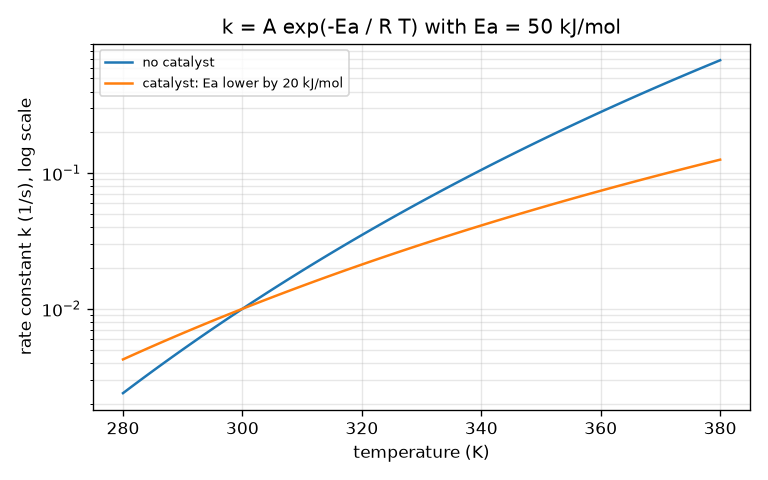
\includegraphics[width=0.85\linewidth]{figures/s02_arrhenius_catalyst.png}\\\small Rate constant against temperature on a log scale: lowering Ea by 20 kJ/mol moves the line up by about 3000 times at 300 K.\end{center}

\subsection*{E. Worked example}
A first-order reaction has k = 0.02 1/s at 300 K. How long does it take to convert 90 percent? How long at 310 K if Ea = 50 kJ/mol, and how long at 300 K with a catalyst that lowers Ea by 5 kJ/mol? What would a drop of 20 kJ/mol give?
\begin{enumerate}[nosep]
\item At 300 K: t = ln(10) / k = 2.303 / 0.02 = 115.1 s.
\item At 310 K: k(310)/k(300) = exp[-(50000/8.314)(1/310 - 1/300)] = exp(0.6463) = 1.909, so k = 0.0382 1/s and t = 2.303 / 0.0382 = 60.3 s.
\item Catalyst, dEa = 5 kJ/mol at 300 K: factor = exp(5000 / (8.314 * 300)) = exp(2.005) = 7.42, so k = 0.148 1/s and t = 15.5 s.
\item Catalyst, dEa = 20 kJ/mol: factor = exp(20000 / (8.314 * 300)) = exp(8.018) = about 3037, so t = 115.1 / 3037 = 0.038 s.
\item Sense check: 10 K warmer gave a factor of 1.9, close to the rule of thumb 'about 2', but a drop of only 5 kJ/mol in the barrier gives 7.4 times: the catalyst is far more powerful than a small warming.
\end{enumerate}
\textbf{Answer.} 115.1 s at 300 K; 60.3 s at 310 K; 15.5 s with a 5 kJ/mol catalyst; and a 20 kJ/mol drop speeds the reaction up about 3000 times (0.038 s).

\subsection*{F. Questions}
\begin{enumerate}[nosep]
\item \textbf{Conceptual.} Why does a catalyst make a reaction faster but not change how much product you finally get (for a reaction that goes to completion)?
\item \textbf{Numerical.} For k = 0.02 1/s at 300 K and Ea = 50 kJ/mol, find k at 320 K. By what factor does it grow?
\item \textbf{Graph and simulation interpretation.} A student plots ln[A] against t and gets a curve bending upwards, while 1/[A] against t is a straight line of slope 0.05 L/(mol s). What is the order and the rate constant? With A0 = 0.5 mol/L what is the half-life?
\item \textbf{Design and optimisation challenge.} Design: a second-order reaction with k = 0.02 L/(mol s) at 300 K and A0 = 1.0 mol/L takes 450 s to reach 90 percent. You need 100 s. Give three ways, with numbers, and discuss the trade-offs.
\end{enumerate}

\section{Session 3: Reaction networks as ODEs, and when they bite back}

\subsection*{A. Real-world problem}
In a real flask many steps happen together: A turns into B, B can turn back, B turns into C; an enzyme grabs a substrate, lets it go or turns it into product. Which step limits how much product you get after a given time? Does a catalyst help if you put it on the wrong step? And what happens to a computer simulation when one step is ten thousand times faster than another? (Simplified teaching models; not for designing a real process.)

\subsection*{B. Concept and theory}
Collect the concentrations of all species in a vector c. Each reaction j has a rate r\_j(c) (for example k [A] for a first-order step, or k1 [E][S] for a binding step). The stoichiometry matrix S has one row per species and one column per reaction: S[i, j] is how many molecules of species i are made (+) or used (-) each time reaction j happens once. Then dc/dt = S r(c), the whole network in one equation. To solve it we step in time with Runge-Kutta 4 (RK4): four slope evaluations per step, error shrinking like h to the fourth power. For first-order networks the equation is linear, dc/dt = K c, and the exact answer c(t) = V exp(L t) V\textasciicircum{}(-1) c0 follows from the eigenvalues of K, which gives a trusted reference. Quantities that every reaction leaves alone are conserved (for E + S \textless{}-\textgreater{} ES -\textgreater{} E + P: E + ES and S + ES + P); they make a good test of the code. If there is little enzyme compared with substrate the complex ES stays almost constant after a short start, and the cycle collapses to the Michaelis-Menten rate v = Vmax [S] / (Km + [S]) with Vmax = k2 E0 and Km = (km1 + k2) / k1 (the quasi-steady-state approximation, QSSA). In a chain the slowest step is the bottleneck. Finally, when rate constants differ by a factor of 10000, the system is stiff: an explicit solver needs a step h with h times the fastest rate below about 2.8, however smooth the answer looks, and above that it blows up; an implicit method (backward Euler) stays stable for any step.

\begin{itemize}[nosep]
\item c: vector of concentrations (mol/L)
\item r(c): vector of reaction rates (mol/(L s))
\item S: stoichiometry matrix (species by reactions) (no unit)
\item K: rate matrix of a first-order network, dc/dt = K c (1/s)
\item h: time step of the solver (s)
\item k1, km1, k2: binding, unbinding and product-forming rate constants of the enzyme cycle (L/(mol s), 1/s, 1/s)
\item E0, S0: total enzyme and starting substrate (mol/L)
\item Vmax, Km: Michaelis-Menten maximum rate and constant (mol/(L s), mol/L)
\end{itemize}

\begin{equation*}
\frac{d\mathbf c}{dt}=S\,\mathbf r(\mathbf c)
\end{equation*}

\begin{equation*}
\mathbf c_{n+1}=\mathbf c_n+\frac h6\left(\mathbf k_1+2\mathbf k_2+2\mathbf k_3+\mathbf k_4\right)\quad(\text{RK4})
\end{equation*}

\begin{equation*}
v=\frac{V_{\max}[S]}{K_m+[S]},\qquad V_{\max}=k_2E_0,\qquad K_m=\frac{k_{-1}+k_2}{k_1}
\end{equation*}

\begin{equation*}
[E]+[ES]=E_0,\qquad [S]+[ES]+[P]=S_0
\end{equation*}

\begin{equation*}
\text{explicit RK4 is stable only if }h\,k_{\text{fast}}\lesssim 2.8;\qquad (I-hK)\,\mathbf c_{n+1}=\mathbf c_n\ \ (\text{backward Euler})
\end{equation*}

\begin{center}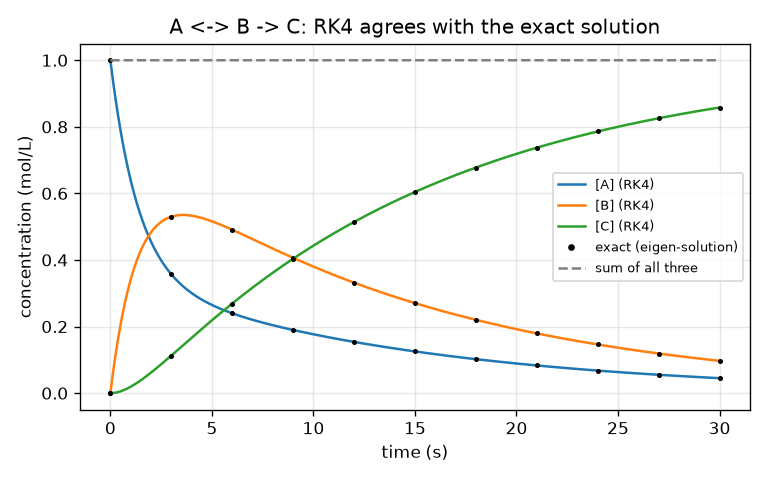
\includegraphics[width=0.85\linewidth]{figures/s03_abc_network.png}\\\small A \textless{}-\textgreater{} B -\textgreater{} C: RK4 (lines) against the exact eigen-solution (dots) and the sum of the three species (dashed).\end{center}

\subsection*{E. Worked example}
For the enzyme cycle with k1 = 10 L/(mol s), km1 = 5 1/s, k2 = 1 1/s and E0 = 0.1 mol/L, find Km and Vmax and the Michaelis-Menten rate at S = 1.0 mol/L. Then compare with the full model.
\begin{enumerate}[nosep]
\item Km = (km1 + k2) / k1 = (5 + 1) / 10 = 0.6 mol/L.
\item Vmax = k2 E0 = 1 * 0.1 = 0.1 mol/(L s).
\item v(S = 1.0) = Vmax S / (Km + S) = 0.1 * 1.0 / 1.6 = 0.0625 mol/(L s). At S = Km the rate would be Vmax / 2 = 0.05.
\item Run the full four-species RK4 (h = 0.005 s). At t = 1 s the model has S = 0.8837 mol/L and ES = 0.05967 mol/L, so the true product rate k2 [ES] = 0.05967 mol/(L s).
\item The QSSA rate at that same S is 0.1 * 0.8837 / (0.6 + 0.8837) = 0.05956 mol/(L s), within 0.2 percent of the full model. The conserved sums E + ES = 0.1 and S + ES + P = 1.0 hold to 1e-14.
\end{enumerate}
\textbf{Answer.} Km = 0.6 mol/L, Vmax = 0.1 mol/(L s), v(1.0) = 0.0625 mol/(L s); at 1 s the full model gives 0.05967 and the QSSA 0.05956 mol/(L s), and both conserved sums stay constant.

\subsection*{F. Questions}
\begin{enumerate}[nosep]
\item \textbf{Conceptual.} Why is it useful that the sum of the concentrations (or E + ES and S + ES + P) stays constant in a simulation? What would it tell you if one drifted?
\item \textbf{Numerical.} For E0/S0 = 0.1 and 1.0 the largest QSSA error in the product is 0.022 and 0.201 times S0. For which ratio would you trust the Michaelis-Menten equation to within 1 percent of S0? How can you check without running the full model?
\item \textbf{Graph and simulation interpretation.} On the stiffness graph, explicit RK4 with h = 1e-3 blows up and h = 1e-4 does not. Explain the numbers using the fastest rate constant 10000 1/s and the limit h k of about 2.8.
\item \textbf{Design and optimisation challenge.} Design: in the chain A -\textgreater{} B -\textgreater{} C -\textgreater{} D with k = 0.8, 0.05 and 0.6 1/s a catalyst can speed up only one step. You want the yield of D at 10 s to at least double (0.295 to 0.59 mol/L). Which step, and what factor? Why can the other two steps not do it?
\end{enumerate}

\section{Real-world mini-project}
\textbf{Which step should the catalyst speed up?.} A plant makes D in a chain A -\textgreater{} B -\textgreater{} C -\textgreater{} D with rate constants 0.8, 0.05 and 0.6 per second, starting from 1 mol/L of A and no B, C or D. After 10 s the yield of D is only about 0.295 mol/L. The chemist can make exactly one step faster with a catalyst. Using \texttt{chain\_yield} and \texttt{speed\_up\_one} from Session 3, find which single step to speed up so that the yield of D after 10 s doubles, and the smallest speed-up factor (searching up to 1000 times) that does it. General education only: real catalyst choice needs experiments and safety review.

\section{The path ahead}
\begin{enumerate}[nosep]
\item \textbf{Session 4: Temperature-dependent networks.} A network simulator in which every step has an activation energy and the temperature is an input.
\item \textbf{Session 5: Fit rate constants from noisy data.} A fitting routine that recovers k1 and k2 of A -\textgreater{} B -\textgreater{} C from synthetic data.
\item \textbf{Session 6: Heat of reaction: exothermic and endothermic.} An adiabatic reactor in which the heat released changes k, with the catalyst as a switch.
\item \textbf{Session 7: An implicit solver for stiff nonlinear networks.} A stiff solver that handles the enzyme cycle with k1 = 1e6 L/(mol s).
\item \textbf{Session 8: Oscillating reactions.} A Brusselator simulation with a stability picture.
\end{enumerate}

\section{Answers and hints}

\subsection*{Session 1}
\begin{enumerate}[nosep]
\item \textbf{Conceptual.} Hint: What does the rate depend on, and what happens to that quantity as time goes on? Solution: The rate is k [A]. At the start there is a lot of A, so many reactions happen per second. As A is used up there are fewer A molecules and fewer collisions, so the rate falls and the curve flattens. The rate constant k itself is unchanged; the rate falls only because [A] falls.
\item \textbf{Numerical.} Hint: k t = 1 after 20 s. Use [A] = A0 exp(-k t) and t\_half = ln 2 / k. Solution: [A] = 2.0 * exp(-1) = 0.736 mol/L. Half-life = 0.693 / 0.05 = 13.9 s. Sense check: 20 s is about 1.44 half-lives, so [A] should be 2.0 * 0.5\textasciicircum{}1.44 = 0.736. They agree. Units: concentration in mol/L, k in 1/s.
\item \textbf{Graph and simulation interpretation.} Hint: They cross when [A] = [B], that is when exactly half of A has reacted. Solution: They cross at the half-life, 6.9 s, at the value 0.5 mol/L (half of A0). With A0 = 2 they would cross at the same time, 6.9 s, but at 1.0 mol/L, because the half-life of this reaction does not depend on the starting concentration.
\item \textbf{Design and optimisation challenge.} Hint: Solve ln(10) / k\_new = 10 s for k\_new, then divide by 0.10. Solution: k\_new = ln(10) / 10 = 0.230 1/s, a factor of 2.3. The next whole number is 3, giving k = 0.30 1/s and a time of 7.7 s with some margin. Other things that matter: cost of the catalyst, whether it can be separated from the product, whether it is poisoned or used up, whether the product is safe, and whether the reaction releases heat that must be removed.
\end{enumerate}

\subsection*{Session 2}
\begin{enumerate}[nosep]
\item \textbf{Conceptual.} Hint: Think of the energy hill between reactants and products: what does the catalyst change, and what stays the same? Solution: A catalyst lowers the height of the hill (the activation energy) by offering a different route. The energy of the reactants and of the products is the same with or without it, so the overall energy change is unchanged, and the reaction still ends at the same place. Only the speed at which it gets there changes, because the rate constant is larger.
\item \textbf{Numerical.} Hint: Use k(T2)/k(T1) = exp[-(Ea/R)(1/T2 - 1/T1)] with T in kelvin. Solution: Factor = exp[-(50000/8.314)(1/320 - 1/300)] = exp[6014 * 0.0002083] = exp(1.2529) = 3.50. k(320) = 0.02 * 3.50 = 0.070 1/s. Check: two steps of 10 K at about 1.9 each is 1.9 * 1.9 = 3.6, close. Units: 1/s.
\item \textbf{Graph and simulation interpretation.} Hint: Which plot is straight tells the order; the slope of that straight line is k. Solution: 1/[A] straight means second order, and the slope is k = 0.05 L/(mol s). Half-life = 1 / (k A0) = 1 / (0.05 * 0.5) = 40 s. The ln[A] plot is curved because ln[A] is only straight for first order.
\item \textbf{Design and optimisation challenge.} Hint: t = x / (k A0 (1 - x)) = 9 / (k A0) for x = 0.9. Need k A0 = 0.09 L/s. Use dEa = R T ln(factor) and T from the Arrhenius ratio (Ea = 50 kJ/mol). Solution: k A0 must rise by a factor of 4.5. (1) Raise the concentration to A0 = 4.5 mol/L: t = 9 / (0.02 * 4.5) = 100 s, but that uses 4.5 times more material and may not dissolve. (2) A catalyst with dEa = R T ln 4.5 = 8.314 * 300 * 1.504 = 3.75 kJ/mol. (3) Heat: 1/T = 1/300 - R ln(4.5)/50000 gives T = 324 K (about 51 degrees C). Trade-offs: heating costs energy and may speed side reactions or damage a product; a catalyst has to be bought and separated; concentration is limited by solubility and by heat release.
\end{enumerate}

\subsection*{Session 3}
\begin{enumerate}[nosep]
\item \textbf{Conceptual.} Hint: Think about atoms that cannot be created or destroyed, and about numerical mistakes. Solution: Reactions only rearrange the same atoms, so these sums must not change; they are built into the structure of S (every column of S for A \textless{}-\textgreater{} B -\textgreater{} C sums to zero). In a simulation they give a free test: if a sum drifts, there is a bug in the rate equations or S, or the step is too large and the numerical error is big. Passing the test does not prove that the rates are right, but failing it proves something is wrong.
\item \textbf{Numerical.} Hint: Look at the trend: the error grows about in proportion to E0/S0. A rule of thumb is E0 much smaller than S0 + Km. Solution: The error is roughly 0.2 times the ratio, so under 1 percent of S0 needs a ratio of about 0.04 or less (the lesson gives 0.0067 at 0.03 and 0.0022 at 0.01). A quick rule without the full model: the approximation needs E0 much smaller than S0 + Km (here 1.6 mol/L), which is why E0 = 0.1 mol/L works well and E0 = 1.0 mol/L does not.
\item \textbf{Graph and simulation interpretation.} Hint: Compute h times k\_fast for both steps. Solution: For h = 1e-3: h k = 10, above the stability limit 2.8, so every step multiplies the error by a factor larger than one and it explodes (overflow to infinity). For h = 1e-4: h k = 1, below the limit, so it is stable. The true solution is smooth after a few ten-thousandths of a second; the step must be small only to keep the fast, already finished, step stable.
\item \textbf{Design and optimisation challenge.} Hint: Use chain\_yield and speed\_up\_one for each step with a list of factors, then bisection on the best step. Solution: Step 2 (k = 0.05, the slowest, the rate-determining step) with a factor of about 2.62 gives a yield of 0.59. Speeding step 1 or step 3 by 1000 times gives only 0.339 and 0.353: those steps are not the bottleneck and the product is limited by the slow step in the middle, so the yield cannot reach 0.59 whatever you do to them. A 2.62 times faster step 2 corresponds to a drop of about R T ln 2.62 = 2.4 kJ/mol in activation energy at 300 K. Trade-off: the faster step 2 drains B into C; then step 3 (and reverse reactions in real systems) will become the next limit.
\end{enumerate}

\section{How to join}
Read \texttt{CONTRIBUTING.md} in the repository, then pick an issue labelled \texttt{good first issue}. Repository: \url{https://github.com/KrunalPanchal1995/openreactionrate}

\end{document}
